\chapter*{Introduction}
\addcontentsline{toc}{chapter}{Introduction}

\section*{The Worldwide LHC Computing Grid}

In the past decade the scientific research collaborations, as well as the
commercial world, have witnessed the start of a  period  of  explosive
data growth. The expressions like "Data Tsunami" or "Big Data" became widespread
and entered a standard terminology. The scientific collaborations developed a
world leading expertise in building and operating very large scale infrastructures for
handling unprecedented and ever growing volumes of data to be processed and analyzed~\cite{OSC}.  
One of the most important scientific communities,
for which these abilities became essential, is the High Energy Physics (HEP) community of 
the experiments at the Large Hadron
Collider (LHC) at CERN\footnote{European Organization for Nuclear Research 
(name derived from Conseil Européen pour la Recherche Nucléaire) -- European research organization that operates 
the largest particle physics laboratory in the world.}.

Physicists collide particles accelerated to enormous energies to get at very short scales, which enables them to
reveal at the microscopic level the basic ingredients of the matter and their interactions. 
On the edge of our millennium their ultimate instrument is the LHC, colliding protons or 
atomic nuclei. In each 
collision debris of tens of thousands of new particles are created which have to be registered in huge detectors 
and carefully analyzed for signs of new physical phenomena. The collisions take part at four interaction areas, 
where the detectors (ATLAS, ALICE, CMS and LHCb) were built. Each experiment collects huge volumes of data that have
to be stored, remaining accessible to many groups of physicist scattered all around the globe.

The volumes of collected data are larger than
%On the edge of our millennium scientists working on the LHC were expecting enormous volumes 
%of data, larger than 
any single computing center within the LHC collaboration could handle, so the concept of 
distributed data management was conceived. In 2001 the CERN Council approved the start of an international 
collaborative project that consists of a grid-based computer network infrastructure, the Worldwide LHC Computing 
Grid (WLCG)~\cite{happyBday}. 

\begin{wrapfigure}{L}{0.6\textwidth}
\centering
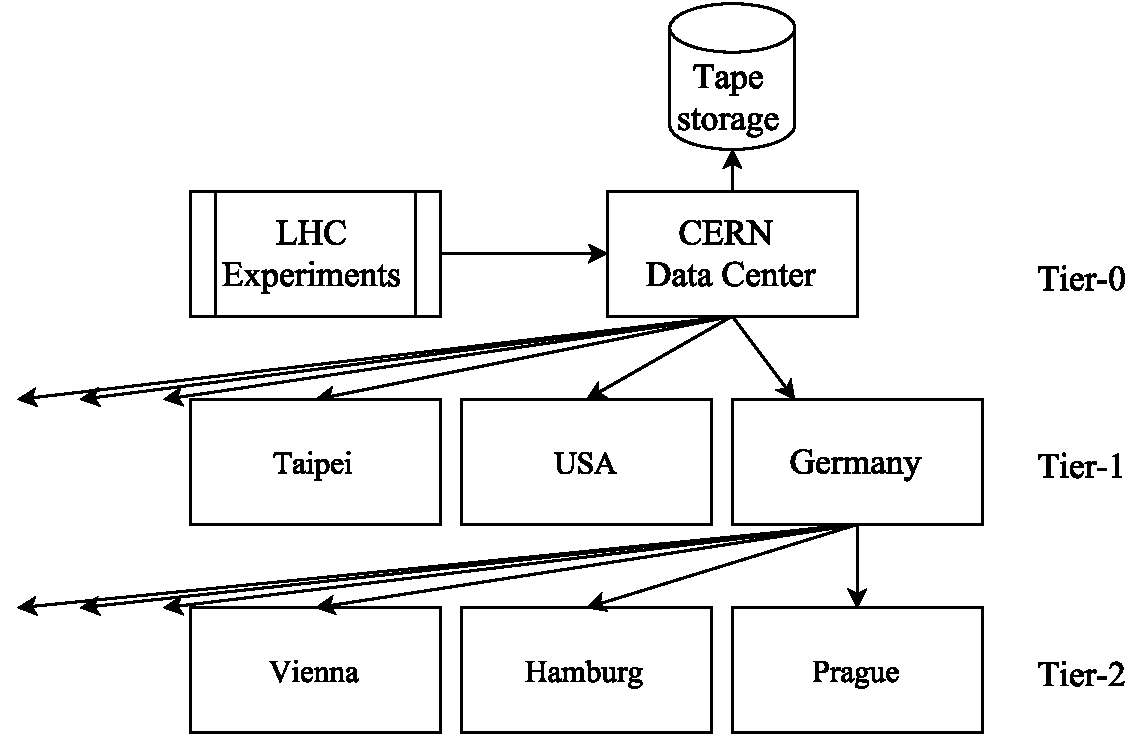
\includegraphics[width=0.55\textwidth]{Tiers.pdf}
\caption{The WLCG Tier-1 centers with CERN Tier-0 in the middle}
\label{fig:WLCG}
\end{wrapfigure}

The WLCG has a hierarchical architecture, where participating sites are categorized -- according to the resources 
and services they provide -- into four importance levels called Tiers. Each Tier is represented by a single or 
distributed computing and storage cluster and yields a specific set of services. The largest center, CERN data 
center or Tier-0, provides the  permanent storage of experimental data and makes the data available for the WLCG 
processing. Although it contributes less than 20\% of the WLCG computing capacity, the role of CERN is unique in 
keeping one copy of the data from all experiments and for performing the first pass of the data reconstruction. 
When LHC is not running, Tier-0 provides resources for re-processing of the raw experimental data and eventually 
for simulation campaigns. 

Another copy is passed to one of the Tier-1 centers. Tier-1s are huge computing centers located in Europe, Canada, USA 
and Taipei. They provide non-stop support for the Grid, store a share of raw data, perform reprocessing and store 
its output. They are connected to CERN with dedicated high-bandwidth optical-fiber links. Then there are more than 
160 Tier-2 centers all around the world. Their role is mainly to run simulation campaigns and end-user analysis. 
Tier-3 centers are small local computing clusters at universities or research institutes and even individual 
PCs~\cite{TGrid}.

\section*{Grid Middleware}

The operation and functionality of WLCG, as well as other Grid systems, is enabled by specific software packages 
and protocols, so-called Grid middleware. It manages the basic domains of the Grid functions: job management, 
data management, security and information services~\cite{GriCom}. The term middleware reflects the specific role 
of this software system: it is a layer between the application area for solving user tasks 
and the resource area consisting of basic fabric and connectivity layer. 

The vast variety of requirements and needs of the user communities from the four LHC experiments is impossible to 
meet with only one set of middleware components. Consequently, each experiment user group started developing its 
own set of tools. For example AliEn is a middleware solution made by the 
ALICE experiment collaboration and DIRAC was developed by the 
LHCb collaboration. Along with some packages from the WLCG-middleware 
they include some additional specific packages and provide complete framework for data processing according to the 
individual experiments' computing models.

\section*{DIRAC}

The DIRAC\footnote{The Distributed Infrastructure with Remote Agent Control} middleware was developed to satisfy
the needs of not only the LHCb collaboration developing it, but also to enable other smaller experiments to use
it as their middleware solution. This was achieved by focusing on modular architecture that enables
adding new features or modifying the systems behavior according to individual experiment's needs. 

DIRAC is constructed from loosely coupled systems where each system manages one part of its functionality. This 
thesis focuses on the DIRAC File Catalog, which is a part of the Data Management system. This particular 
system is responsible for data managing tasks across a wide range of distributed storage elements. It also enables 
users to quickly find and use their files. It is accomplished by maintaining a 
directory structure with a similar interface as the UNIX shell and enabling users to define their own metadata
and use them to search for files.

\section*{Goals of the Thesis}

The first task of this thesis is to upgrade the DIRAC File Catalog (DFC) by:
\begin{itemize}
\item adding a new module for dataset support, enabling users to bundle their files based on a metadata search 
(a~metaquery) into a single object,
\item implementing a class to encapsulate all the methods handling metaquery and to extend its 
functionality by adding normalization and optimization procedures.
\end{itemize}

%\noindent 
The second task is to test the hypothesis that storing the user defined metadata in a suitable NoSQL database 
would improve metaquery performance. If the tests prove that hypothesis, the task is to extend the code of DIRAC 
to incorporate the database in the File Catalog making a prototype, that can be then evaluated by the DIRAC 
collaboration.

\section*{Structure of the Thesis}

In Chapter~\ref{chap:DIRAC} the DIRAC middleware will be introduced with the focus on the data management part and the 
file catalog. Afterwards DIRAC will be compared to two other middleware solutions in Chapter~\ref{chap:relwork}, 
more specifically ATLAS Distributed Data Management system and ALICE Environment framework.

In the next two chapters our contribution to DIRACs code will be presented. The Chapter~\ref{chap:MQ} 
is about the new MetaQuery class and the Chapter~\ref{chap:Dataset} deals with the Dataset Manager.

In the last part several NoSQL databases will be tested in order to select the one that is the best option for storing
file metadata (Chapter~\ref{chap:databases}) and in the Chapter~\ref{chap:NoSQL} a module created for integrating 
that database is described. 

Finally, the Chapter~\ref{chap:user} provides user documentation to all the commands used to interact with the 
CLI\footnote{Command Line Interface}
of the DFC used to control any of the parts that were changed by this project. The last Chapter
summarizes evaluation of the test results and conclusions.